%%%%%%%%%%%%%%%%%%%%%%%%%%%%%%%%%%%%%%%%%%%%%%%%%%%%%%%%%%%%%
%															%
% %CS_383_Assignment1_LaTeX_UML_Document					%
% LaTeX Template											%
% Version 1.0 (2/9/17)										%
%															%
%															%
% author: Adrian Beehner									%
%															%
%															%
% description: LaTeX document that contains memo and		%
%	appendicies for UML diagramming tools					%
%															%
%%%%%%%%%%%%%%%%%%%%%%%%%%%%%%%%%%%%%%%%%%%%%%%%%%%%%%%%%%%%%


% Set Up Document
\documentclass[12pt]{article}
\usepackage{titlesec} 
\usepackage{hyperref}
\usepackage{graphicx}
\usepackage{float}
\usepackage{parskip} % Adds spacing between paragraphs
\usepackage{xcolor} % For setting colors
\usepackage{listings}
\setlength{\parindent}{15pt} % Indent paragraphs
\usepackage[margin=1in]{geometry}

% Make so Picture/floats go at top of page
\makeatletter
\setlength{\@fptop}{0pt}
\makeatother

% set the default code style
\lstset
{
	frame=tb, % draw a frame at the top and bottom of the code block
	tabsize=3, % tab space width
	showstringspaces=false, % don't mark spaces in strings
	numbers=left, % display line numbers on the left
	commentstyle=\color{green}, % comment color
	keywordstyle=\color{blue}, % keyword color
	stringstyle=\color{red} % string color
}

% Make sure hyperlinks for table of contents and website links dont have wierd red box
\hypersetup{
	colorlinks,
	citecolor=black,
	filecolor=black,
	linkcolor=black,
	urlcolor=black
}

\begin{document}
	
	% Set up Manual Indenting
	\setlength{\parindent}{15pt}
	\newcommand{\forceindent}{\leavevmode{\parindent=2em\indent}}
	
	
	%----------------------------------------------------------------------------------------
	%	TABLE OF CONTENTS
	%----------------------------------------------------------------------------------------	
	% Create title Page
	\title{ Design Specification Update \\ Sprint 3}
	\author{Team 3 (Java)}
	\date{}
	\maketitle
	
	% Create Table of Contents
	\tableofcontents
	%Set Table of Content depth
	\setcounter{tocdepth}{3}		% Include \subsubsection in ToC
	% Create new Page
	\newpage
	
	%----------------------------------------------------------------------------------------
	%	APPENDICIES
	%----------------------------------------------------------------------------------------
	%Apendix Section
	\appendix
	
		%----------------------------------------------------------------------------------------
		%	APPENDIX A Content - Sample Code/Work Done
		%----------------------------------------------------------------------------------------
		\section{Changes/Updates}
		\forceindent The changes made to the Design Specification was relatively small. These changes are listed below.
		
			%----------------------------------------------------------------------------------------
			%	Frame Preview Bar
			%----------------------------------------------------------------------------------------
			\subsection {Updating the Diagram for Grid Editor}
			\forceindent The grid editor diagram was updated to reflect the changes made to it, namely a color picker was added to the right side of the Grid Editor, the text was removed from the buttons, and a set of translation buttons was added to shift patterns around on the frame. See figure 1 below.
      
      \begin{figure}[ht!]
        \centering
        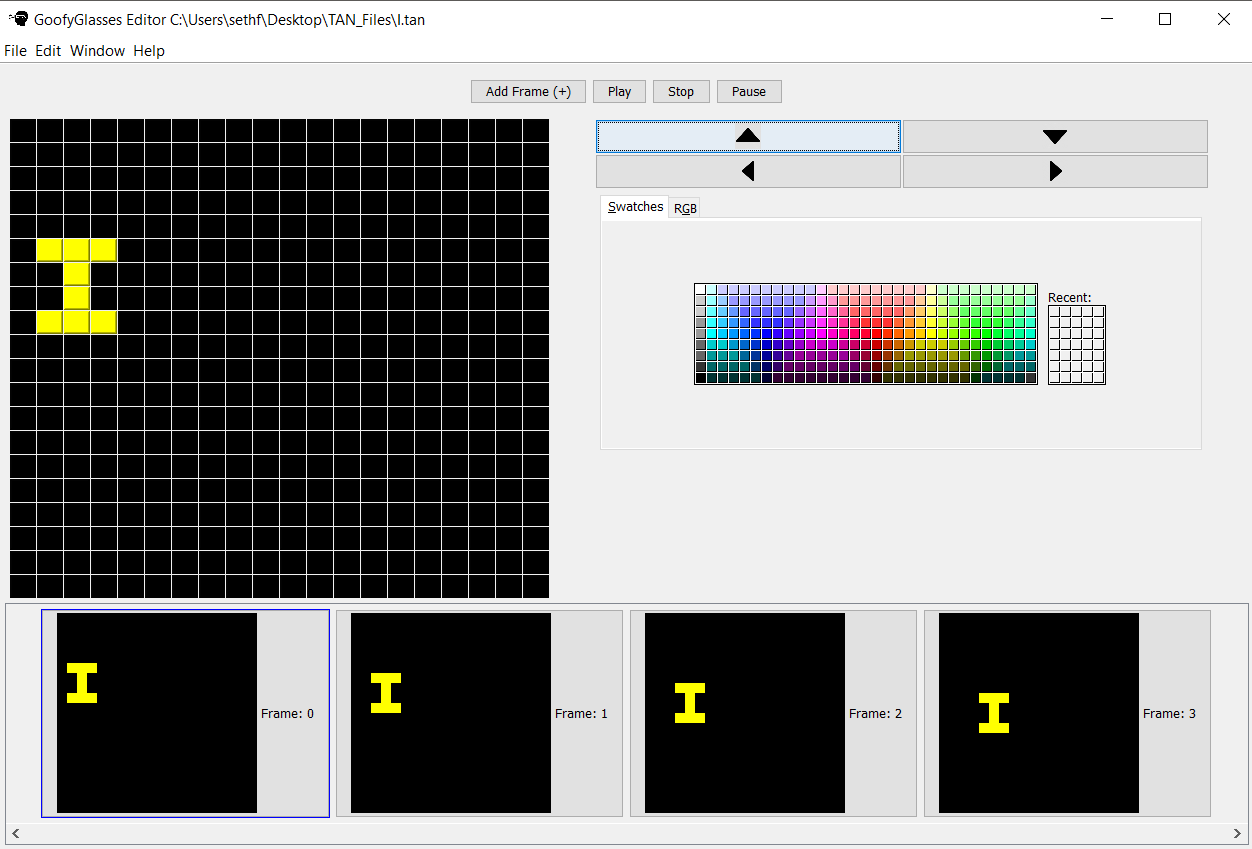
\includegraphics[width=120mm]{gridEditor_ColorPicker.PNG}
        \caption{Diagram of Grid Editor}
      \end{figure}
    
			%----------------------------------------------------------------------------------------
			%	Frame Preview Bar
			%----------------------------------------------------------------------------------------
			\subsection {Updating the Time-line}
			\forceindent The time-line was edited to reflect the progress made since Sprint 2 and also display goals for the following sprint. The time-line now properly indicates the completion and removal of several objectives. It accurately shows that refinements were made to the Grid Editor and the scrub bar, as well as an indication that there will no longer be a multi-node editor. The time-line now also lists the addition of a progress report presentation.
      
			% Create new Page
			\newpage
		
		%----------------------------------------------------------------------------------------
		%	APPENDIX B Content - Sample Code/Work Done
		%----------------------------------------------------------------------------------------
		\section{Updated Section(s)}
		\forceindent The Single and Multi-Node grid editor sections were removed to reflect the change to using a single Grid Editor. These section(s) are further discussed below.
		
		%----------------------------------------------------------------------------------------
		%	Frame Preview Bar
		%----------------------------------------------------------------------------------------
		\subsection {Grid Editor}
		\forceindent The Single and Multi-Node Editor sections were removed to indicate the change in functionality of the design. This new design is a single Grid Editor with a color picker on the side, where there will eventually be the ability to Shift-Click a second node and a section of nodes will be selected to change the color.
    
    \begin{figure}[ht!]
      \centering
      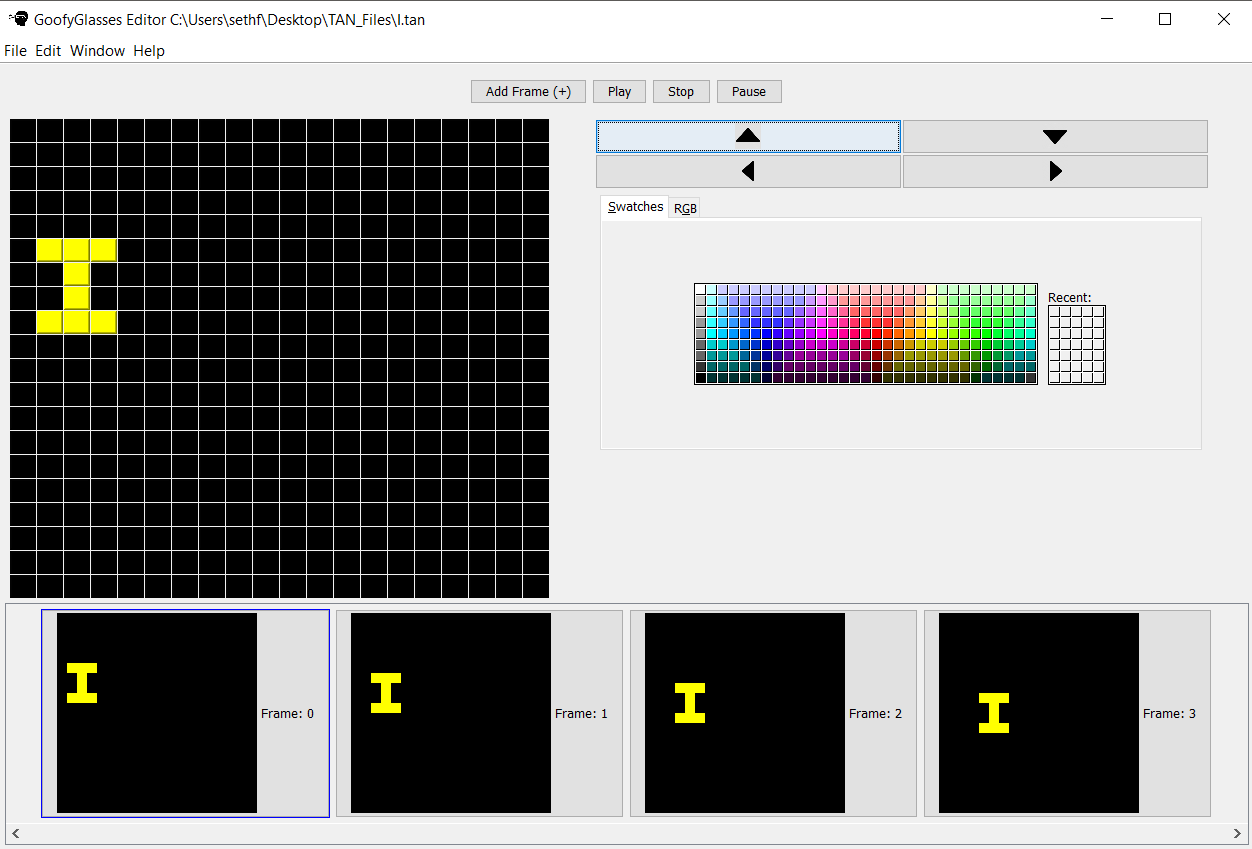
\includegraphics[width=120mm]{gridEditor.PNG}
      \caption{Diagram of Grid Editor}
    \end{figure}
		% Create new Page
		\newpage
		
		%----------------------------------------------------------------------------------------
		\subsection {Frame Preview Bar}
		\forceindent The image below shows the right-click menu on the scrub bar. Most of the functionality is implemented in this menu and it adds a great deal of user-friendlyness to the interface.
		
		\begin{figure}[ht!]
			\centering
				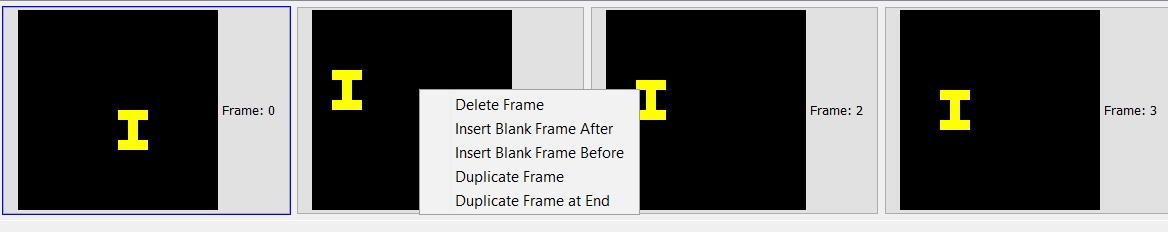
\includegraphics[width=160mm]{rtClick.PNG}
			\caption{Image of the Frame Preview Bar's Right-Click Menu}
		\end{figure}
			
			% Create new Page (NEED TO USE clearpage because we have pictures that will affect it!)
		\clearpage
		
		
\end{document}